\documentclass{article}
\usepackage[utf8]{inputenc}
\usepackage[T1]{fontenc}
\usepackage[ukrainian]{babel}
\usepackage[12pt]{extsizes}
\usepackage{graphicx}
\usepackage{amsmath}
\graphicspath{{pictures/}}
\DeclareGraphicsExtensions{.pdf,.png,.jpg}

\title{Теорвер}
\author{nikita.forduy }
\date{February 2020}

\usepackage{natbib}
\usepackage{graphicx}

\begin{document}
\pagestyle{empty}

\begin{titlepage}
    \thispagestyle{empty}
    \setlength{\parindent}{0ex} % set paragraph indenting to zero
    
    \begin{center}
      НАВЧАЛЬНО-НАУКОВИЙ КОМПЛЕКС \\
      "ІНСТИТУТ ПРИКЛАДНОГО СИСТЕМНОГО АНАЛІЗУ" \\
      НАЦІОНАЛЬНОГО ТЕХНІЧНОГО УНІВЕРСИТЕТУ УКРАЇНИ \\
      "КИЇВСЬКИЙ ПОЛІТЕХНІЧНИЙ ІНСТИТУТ ІМЕНІ ІГОРЯ СІКОРСЬКОГО" \\
      \smallskip
      КАФЕДРА МАТЕМАТИЧНИХ МЕТОДІВ СИСТЕМНОГО АНАЛІЗУ \\
    \end{center}
    \vspace{60mm}
    
    \begin{center}
      РОЗРАХУНКОВА РОБОТА \\
      з предмету "Математична статистика" \\
    \end{center}
    
    \vspace{30mm}
    

    \hfill
    \begin{minipage}{.4\linewidth}
      \begin{flushright}
        Виконав студент групи КА-81
    
        \smallskip
    
        Фордуй Нікіта
      \end{flushright}
    \end{minipage}
    
    \vspace{10mm}

    \vfill
    \begin{center}
      Київ 2020
    \end{center}
    
    \setlength{\parindent}{5ex} % reset paragraph indenting
\end{titlepage}

\pagestyle{plain}

\large
\section{Завдання}
Дана конкретна реалізація вибірки об’ємом n = 100:
\newline
\newline
\begin{tabular}{cccccccccccccccccccc}
  \ttfamily 2 & 0 & 8 & 0 & 15 & 1 & 1 & 1 & 7 & 1 & 0 & 0 & 
  3 & 1 & 1 & 1 & 0 & 0 & 3 & 1 \\
  \ttfamily 2 & 4 & 10 & 6 & 1 & 0 & 1 & 0 & 0 & 2 & 0 & 1 & 
  5 & 0 & 1 & 9 & 4 & 2 & 11 & 3\\
  \ttfamily 2 & 0 & 8 & 1 & 6 & 3 & 0 & 1 & 1 & 4 & 0 & 9 & 
  5 & 3 & 3 & 0 & 0 & 10 & 2 & 0\\
  \ttfamily 3 & 11 & 0 & 9 & 0 & 1 & 4 & 1 & 0 & 2 & 0 & 1 & 
  1 & 3 & 4 & 7 & 1 & 3 & 3 & 0 \\
  \ttfamily 4 & 7 & 6 & 0 & 3 & 0 & 1 & 15 & 11 & 1 & 2 & 4 & 
  0 & 2 & 0 & 0 & 0 & 26 & 4 & 0
\end{tabular}
\newline
\section{Побудова варіаційного ряду вибірки }
Маємо невелику кількість різних значень - тому побудуємо 
дискретний варіаційний ряд.
Підрахувавши кількість варіант (14) та їх частоти і знаючи 
об’єм вибірки отримаємо 
дискретний варіаційний ряд :
\newline
\newline
\begin{tabular}{|l|l|l|l|l|l|l|l|l|l|l|l|l|l|l|}
  \hline
  $x_i^*$& 0 & 1 & 2 & 3 & 4 & 5 & 6 & 7 & 8 & 9 & 10 & 11 & 15 & 26\\
  \hline
  $n_i$& 29 & 22 & 9 & 11 & 8 & 2 & 3 & 3 & 2 & 3 & 2 & 3 & 2 & 1\\
  \hline
  $\omega_i = \frac{n_i}{n}$ & $\frac{29}{100}$ & 
  $\frac{22}{100}$ & $\frac{9}{100}$ & $\frac{11}{100}$ & 
  $\frac{8}{100}$ & $\frac{2}{100}$ & $\frac{3}{100}$ 
  & $\frac{3}{100}$ & $\frac{2}{100}$ & $\frac{3}{100}$ & 
  $\frac{2}{100}$ & $\frac{3}{100}$ & $\frac{2}{100}$ & 
  $\frac{1}{100}$\\
  \hline
\end{tabular}
\newline
\newline
де $x_i^*$ - варіанти реалізації вибірки, $n_i$ - частота 
варіанти, $\omega_i = \frac{n_i}{n}$ - частість варіанти або 
відносна частота.
\newline
\newline
Далі літерою $\xi$ будемо позначати генеральну сукупність, 
реалізацію вибірки якої ми маємо.
\newpage
За дискретним варіаційним рядом побудуємо його геометричну 
інтерпретацію - полігон відносних частот (частостей):
\newline
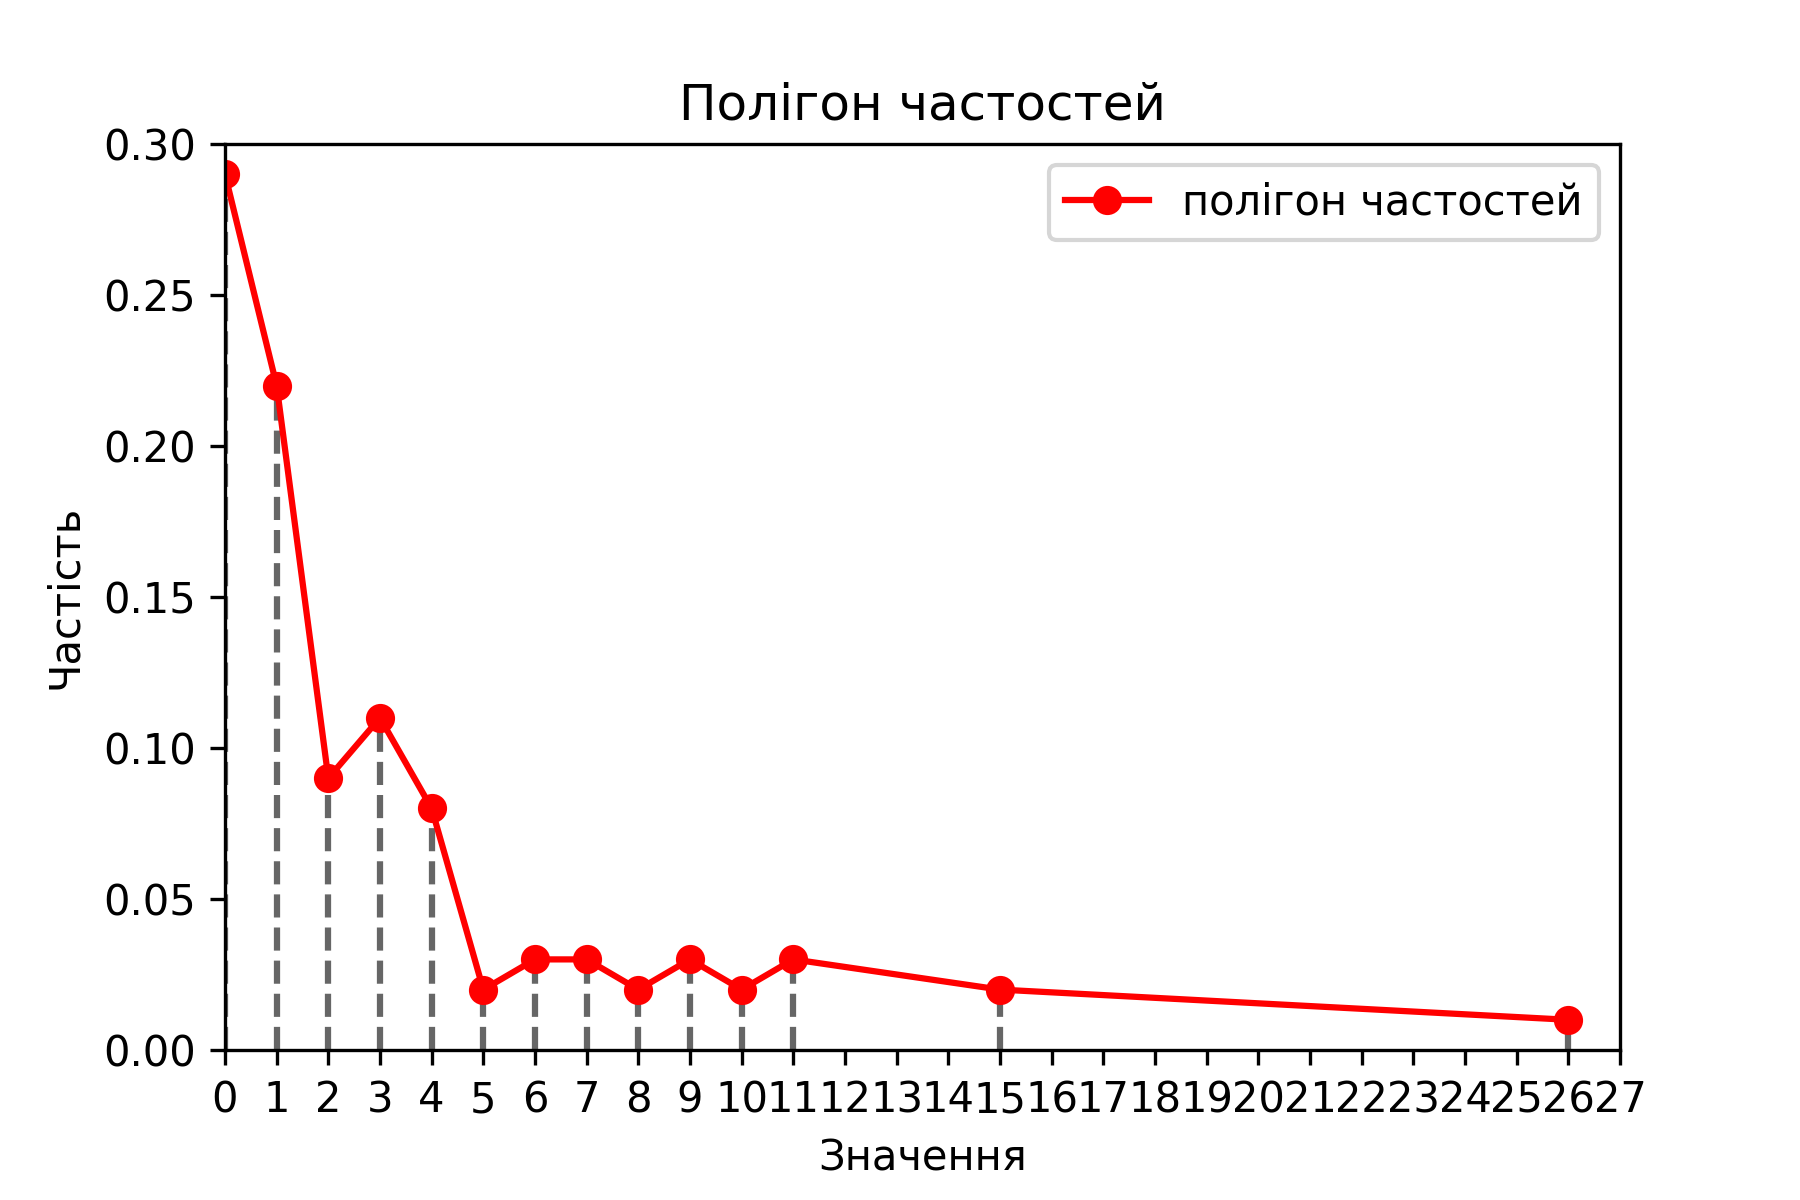
\includegraphics[scale = 0.9]{plot}
\newpage
Порівняємо полігон частостей нашої реалізації 
виборки із полігонами ймовірностей геометричного закону при 
різних значеннях його параметра.
В цьому й наступному розділах мається на увазі геометричний закон
зі значеннями $ \in \{ 0, 1, 2, \dots \} $
\newline
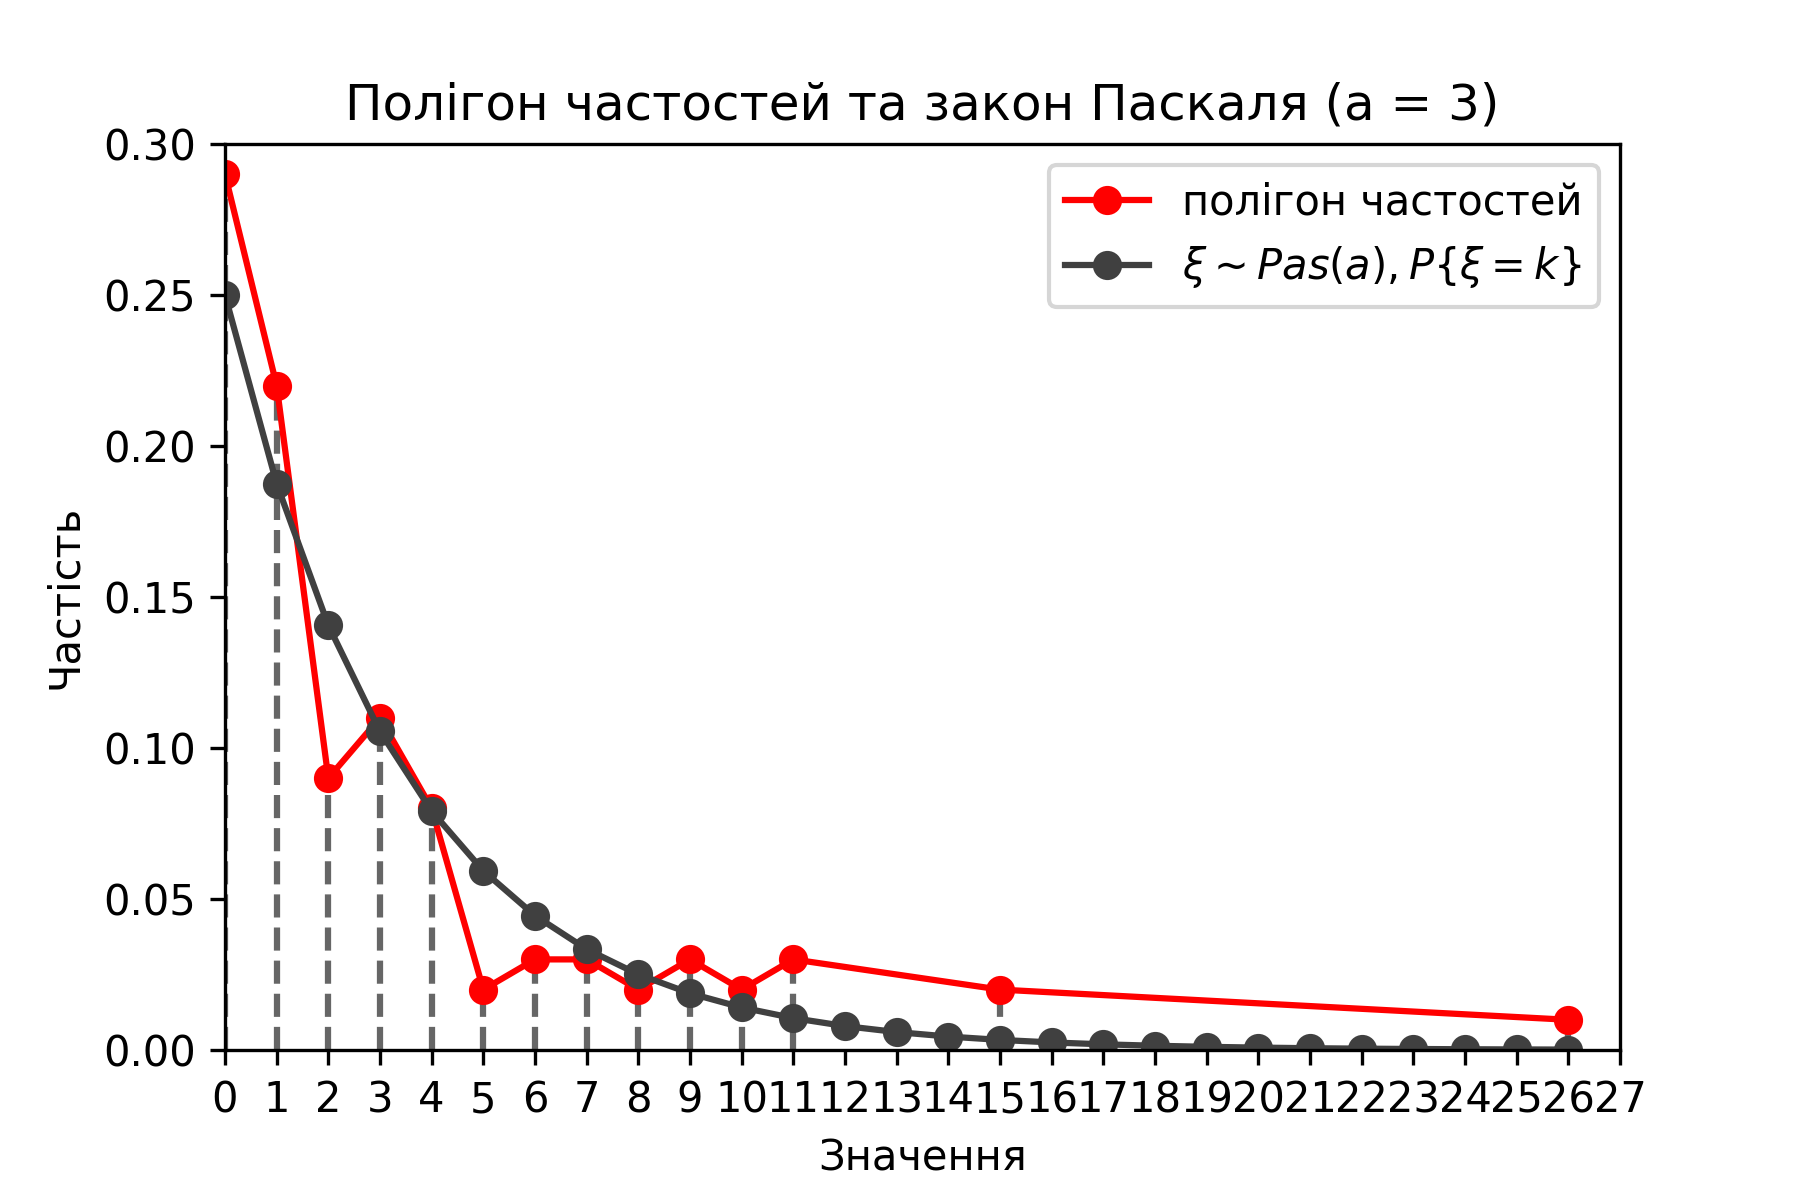
\includegraphics[scale = 0.8]{plot1}
\newline
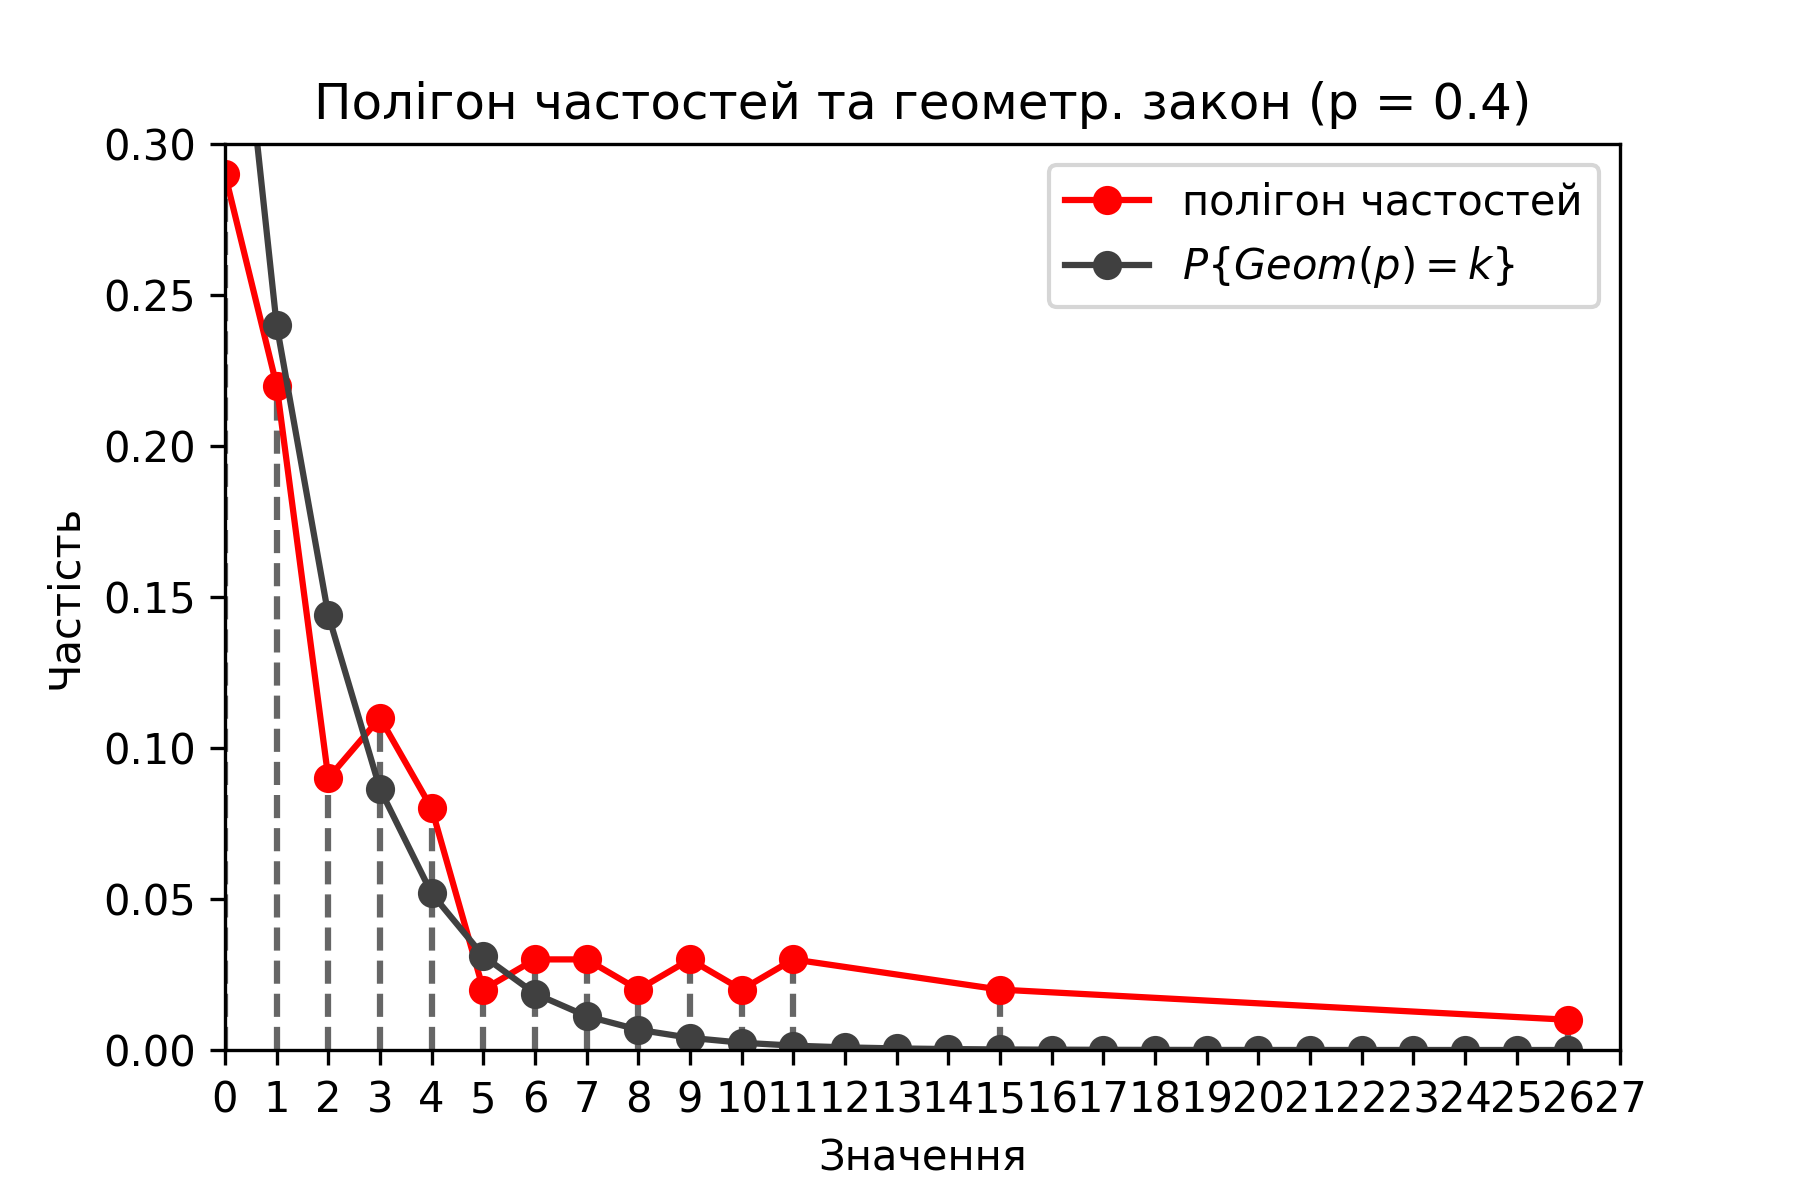
\includegraphics[scale = 0.8]{plot2}
\newline
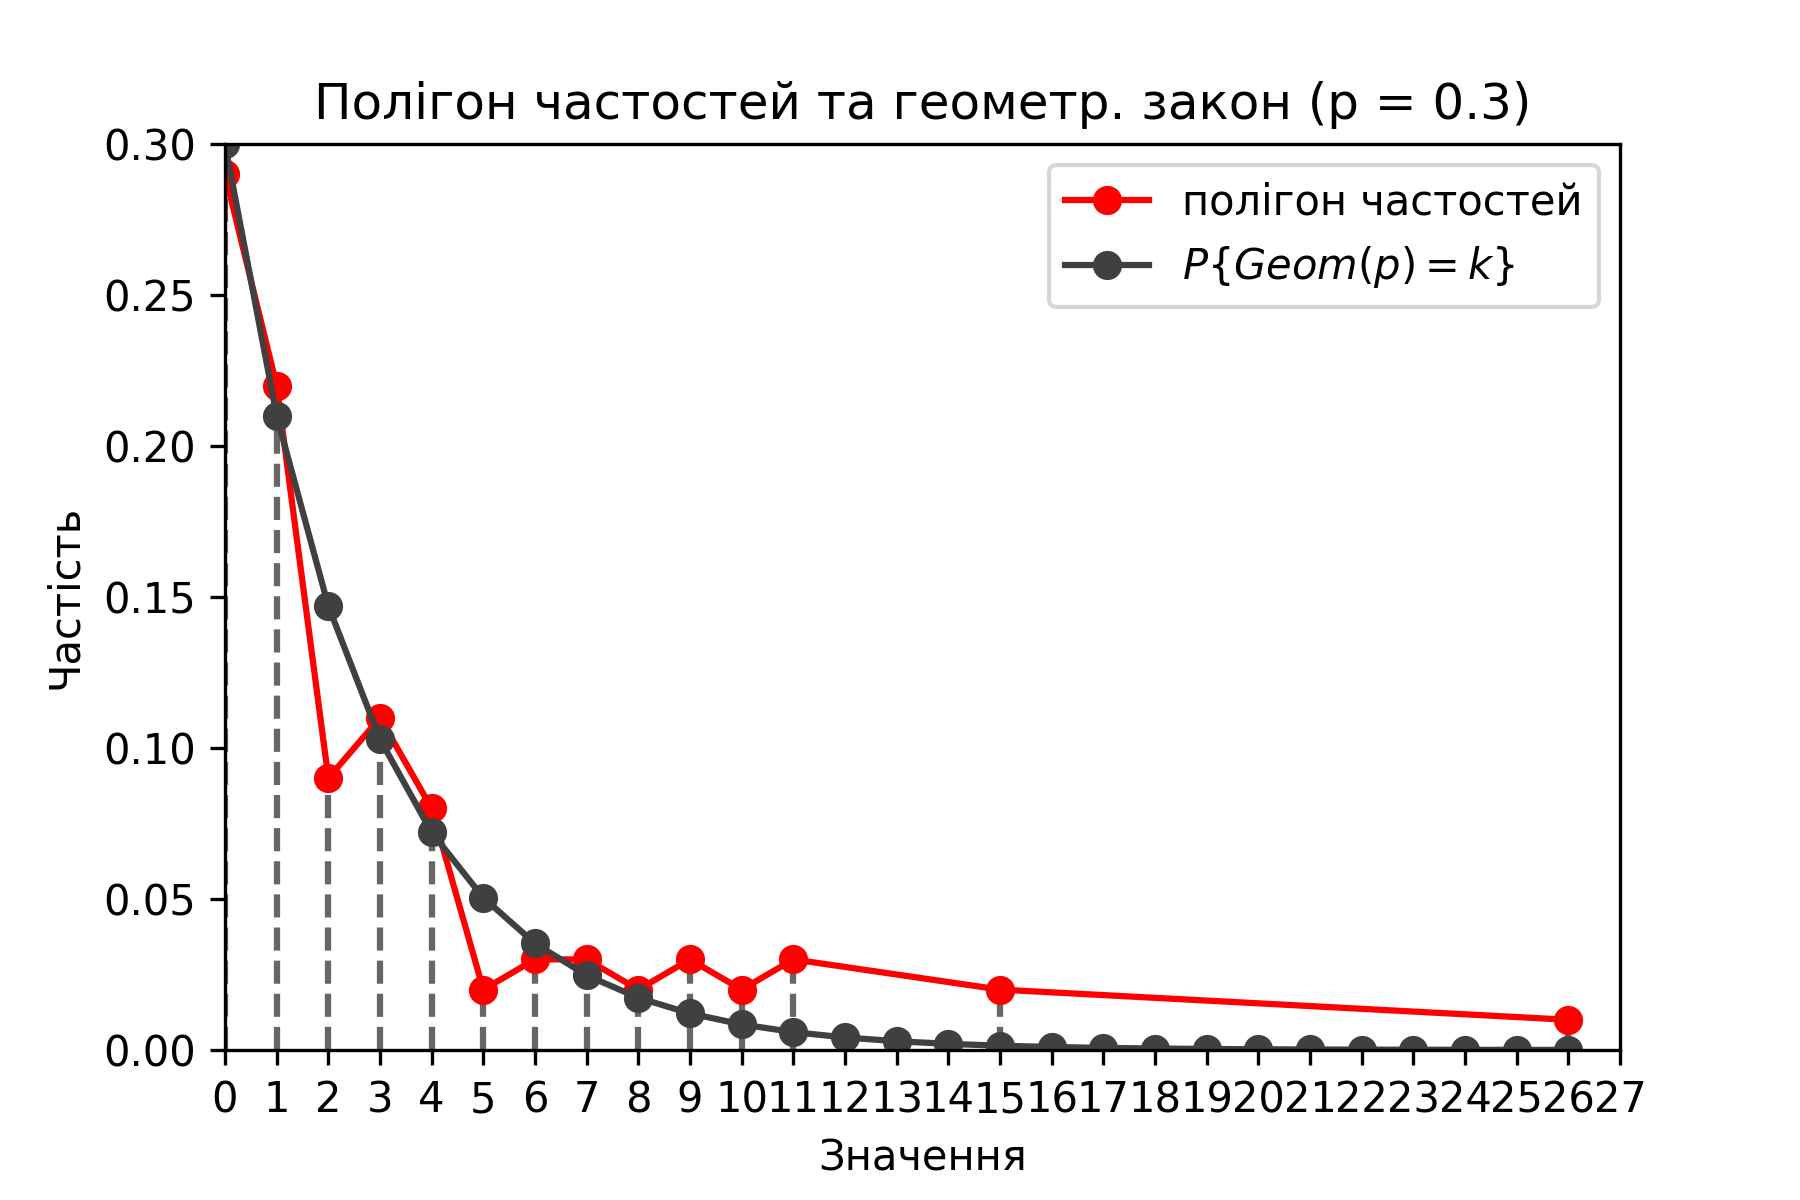
\includegraphics[scale = 0.8]{plot3}
\newline
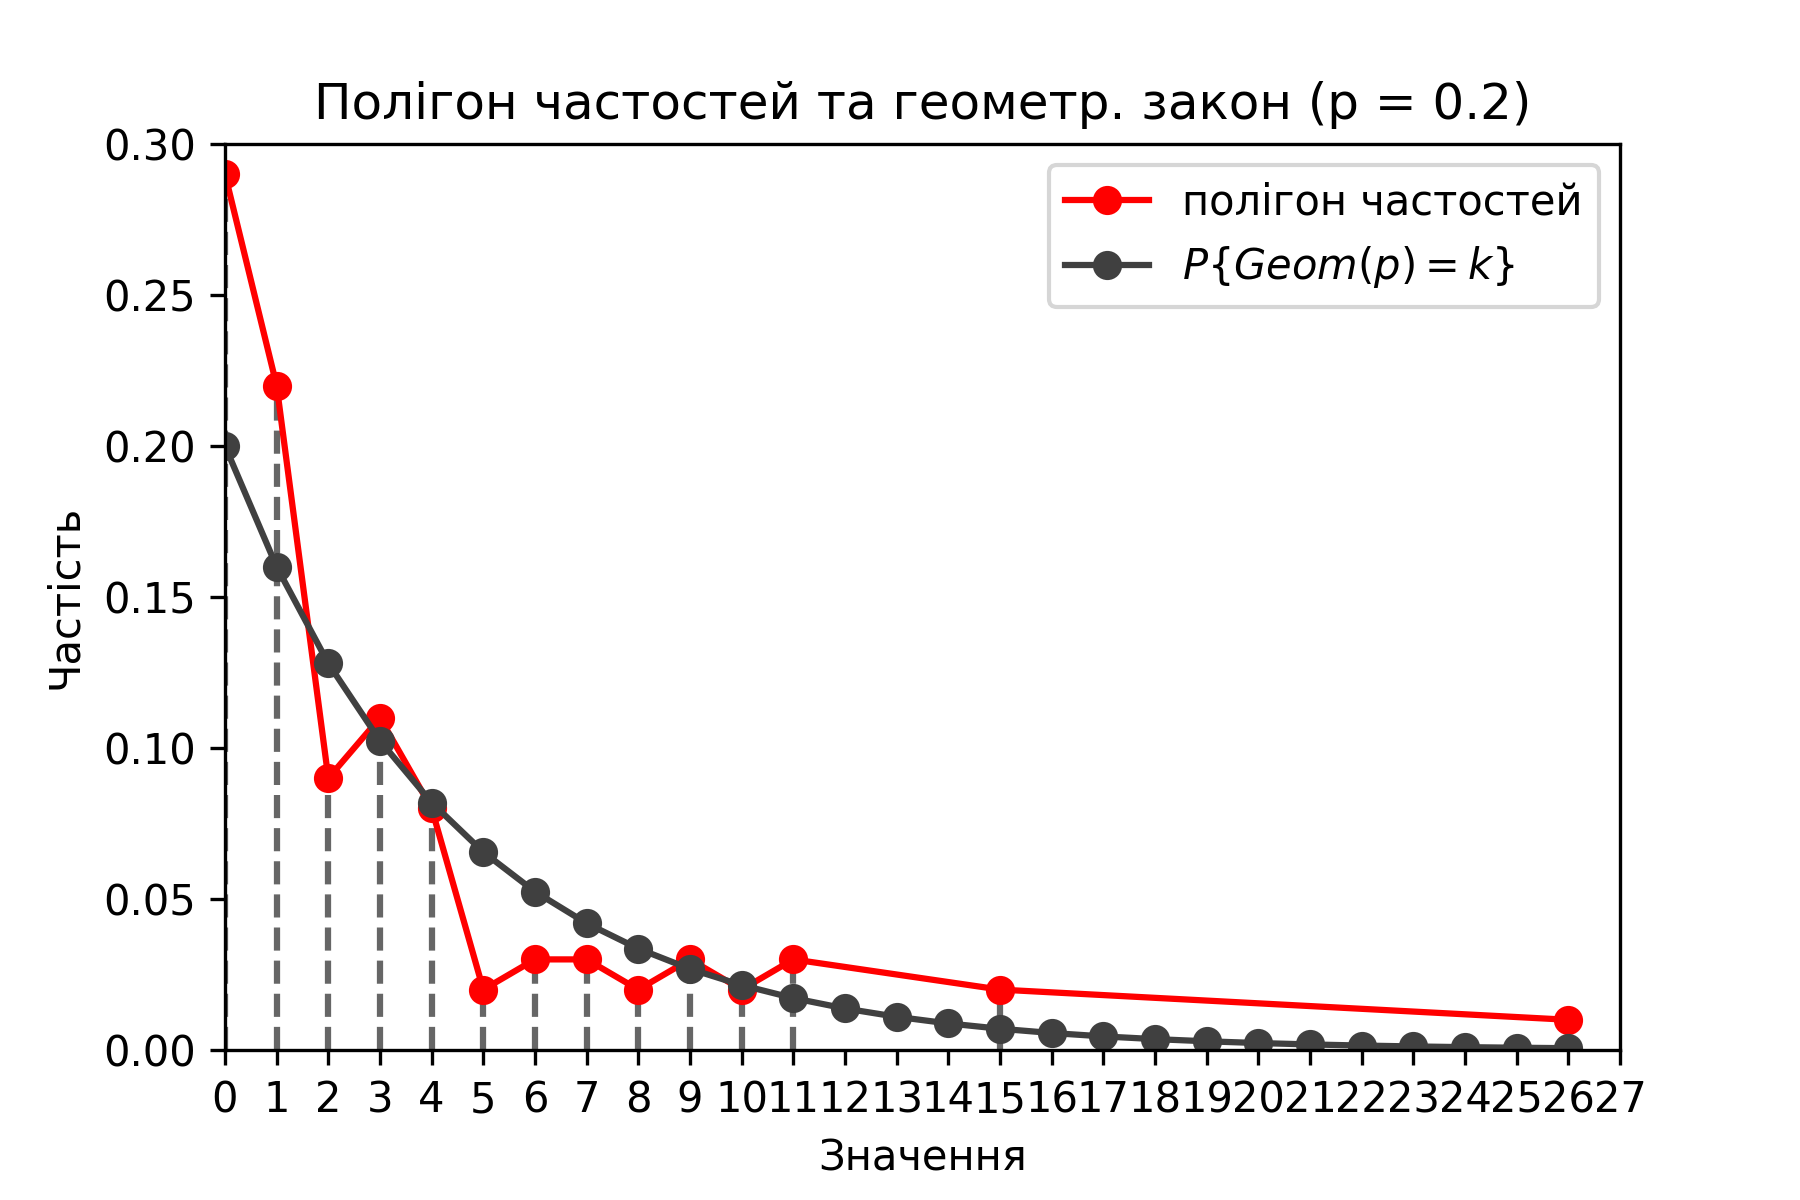
\includegraphics[scale = 0.8]{plot4}
\newline
Можна побачити, що полігон ймовірностей геометричного 
закону при певних значеннях його параметра (p = 0.3, 0.4, 0.5) 
дуже схожий на полігон частостей нашої реалізації вибірки.
\newpage
\section{Емпірична функція розподілу}
Побудуємо емпіричну функцію розподілу за вже побудованим 
дискретним варіаційним рядом:
\newline
$$F_n^*(x) = \begin{cases}
  0,  & x \leq 0 \\
  \frac{29}{100}, & 0 < x \leq 1 \\
  \frac{29 + 22}{100} = \frac{51}{100}, & 1 < x \leq 2 \\
  \frac{51}{100} + \frac{9}{100} = \frac{60}{100}, & 2 < x \leq 3 \\
  \frac{60}{100} + \frac{11}{100} = \frac{71}{100}, & 3 < x \leq 4 \\
  \frac{71}{100} + \frac{8}{100} = \frac{79}{100}, & 4 < x \leq 5 \\
  \frac{79}{100} + \frac{2}{100} = \frac{81}{100}, & 5 < x \leq 6 \\
  \frac{81}{100} + \frac{3}{100} = \frac{84}{100}, & 6 < x \leq 7 \\
  \frac{84}{100} + \frac{3}{100} = \frac{87}{100}, & 7 < x \leq 8 \\
  \frac{87}{100} + \frac{2}{100} = \frac{89}{100}, & 8 < x \leq 9 \\
  \frac{89}{100} + \frac{3}{100} = \frac{92}{100}, & 9 < x \leq 10 \\
  \frac{92}{100} + \frac{2}{100} = \frac{94}{100}, & 10 < x \leq 11 \\
  \frac{94}{100} + \frac{3}{100} = \frac{97}{100}, & 11 < x \leq 15 \\
  \frac{97}{100} + \frac{2}{100} = \frac{99}{100}, & 15 < x \leq 26 \\
  \frac{99}{100} + \frac{1}{100} = 1, & x > 26 \\
\end{cases}$$
\newpage
Зобразимо емпіричну функцію розподілу геометрично :
\newline
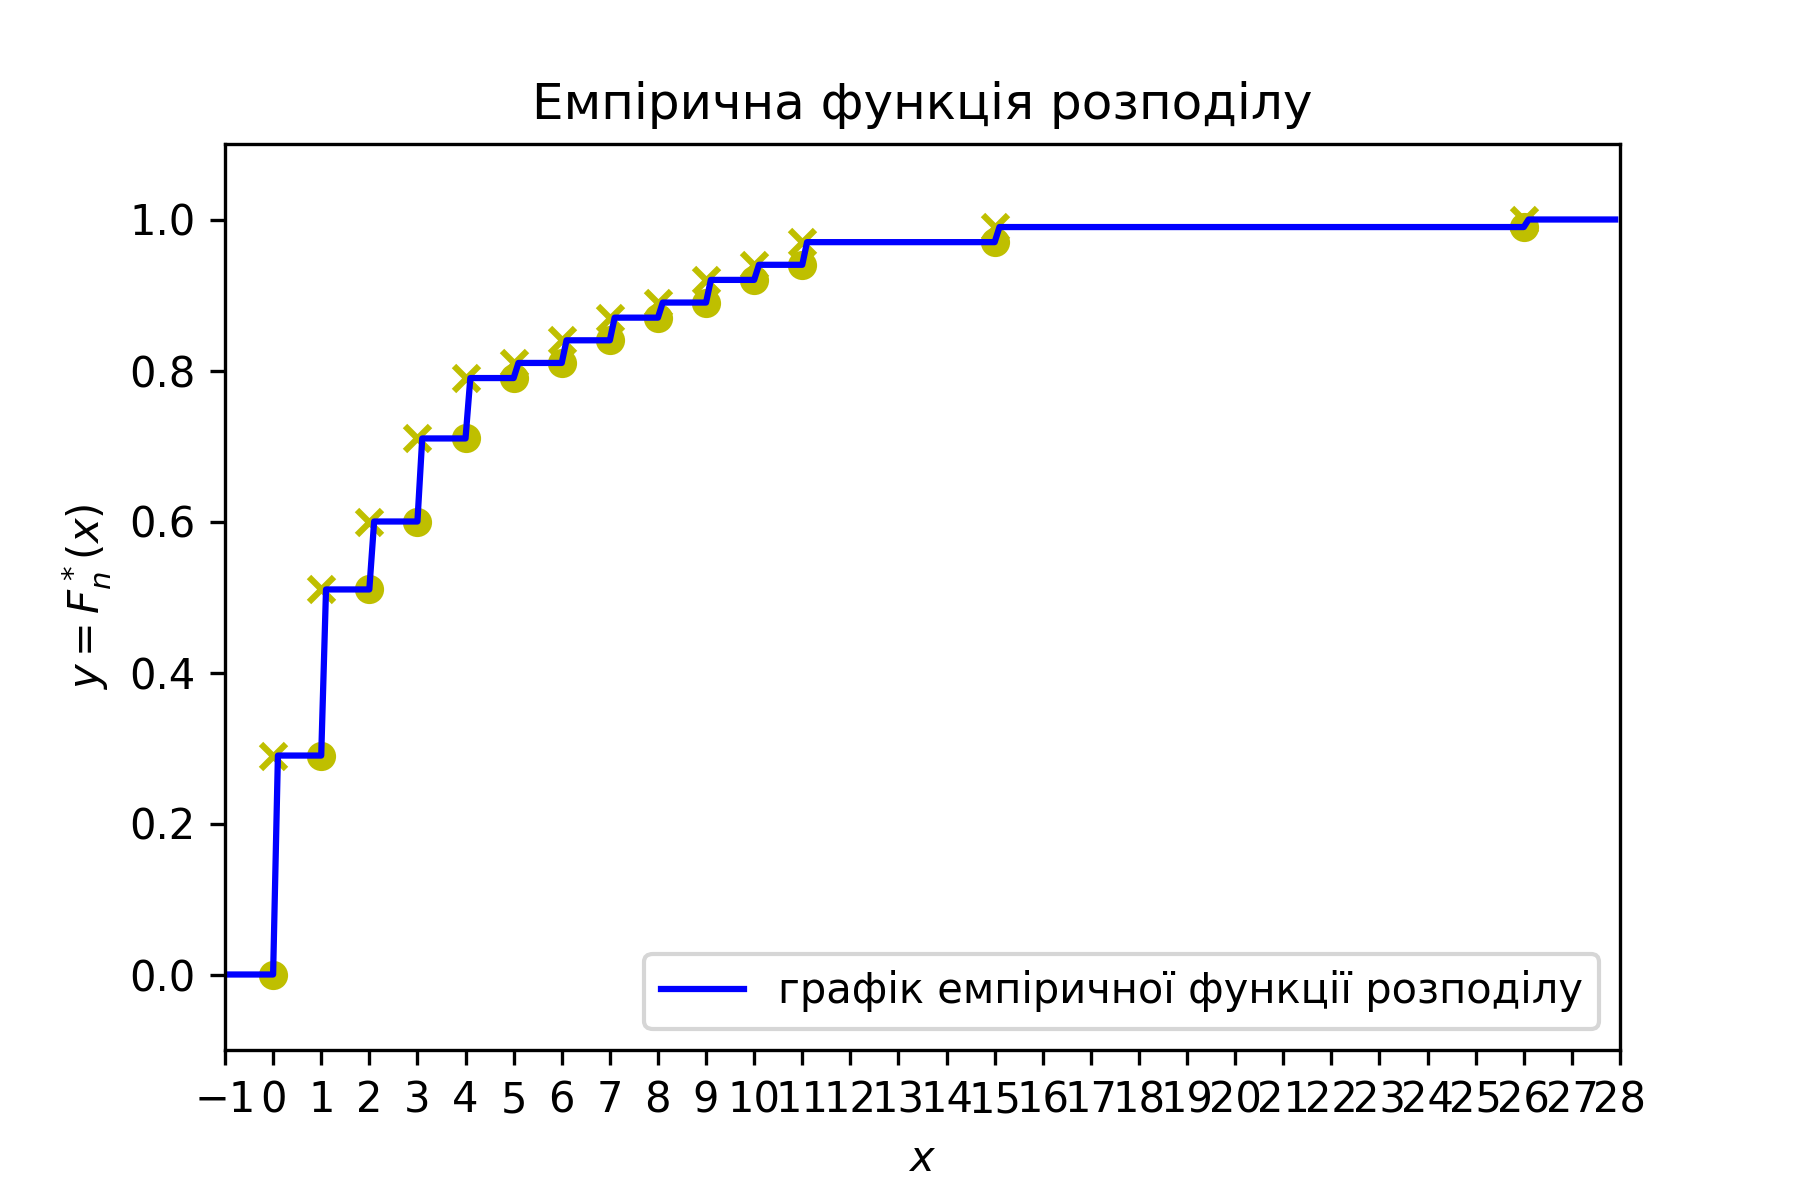
\includegraphics[scale = 0.8]{func}
\newline
Порівняємо графік емпіричної функції розподілу варіаційного ряду 
з графіком функції розподілу геометричного закону при 
різних параметрах(p = 0.4, 0.3, 0.2):
\newline
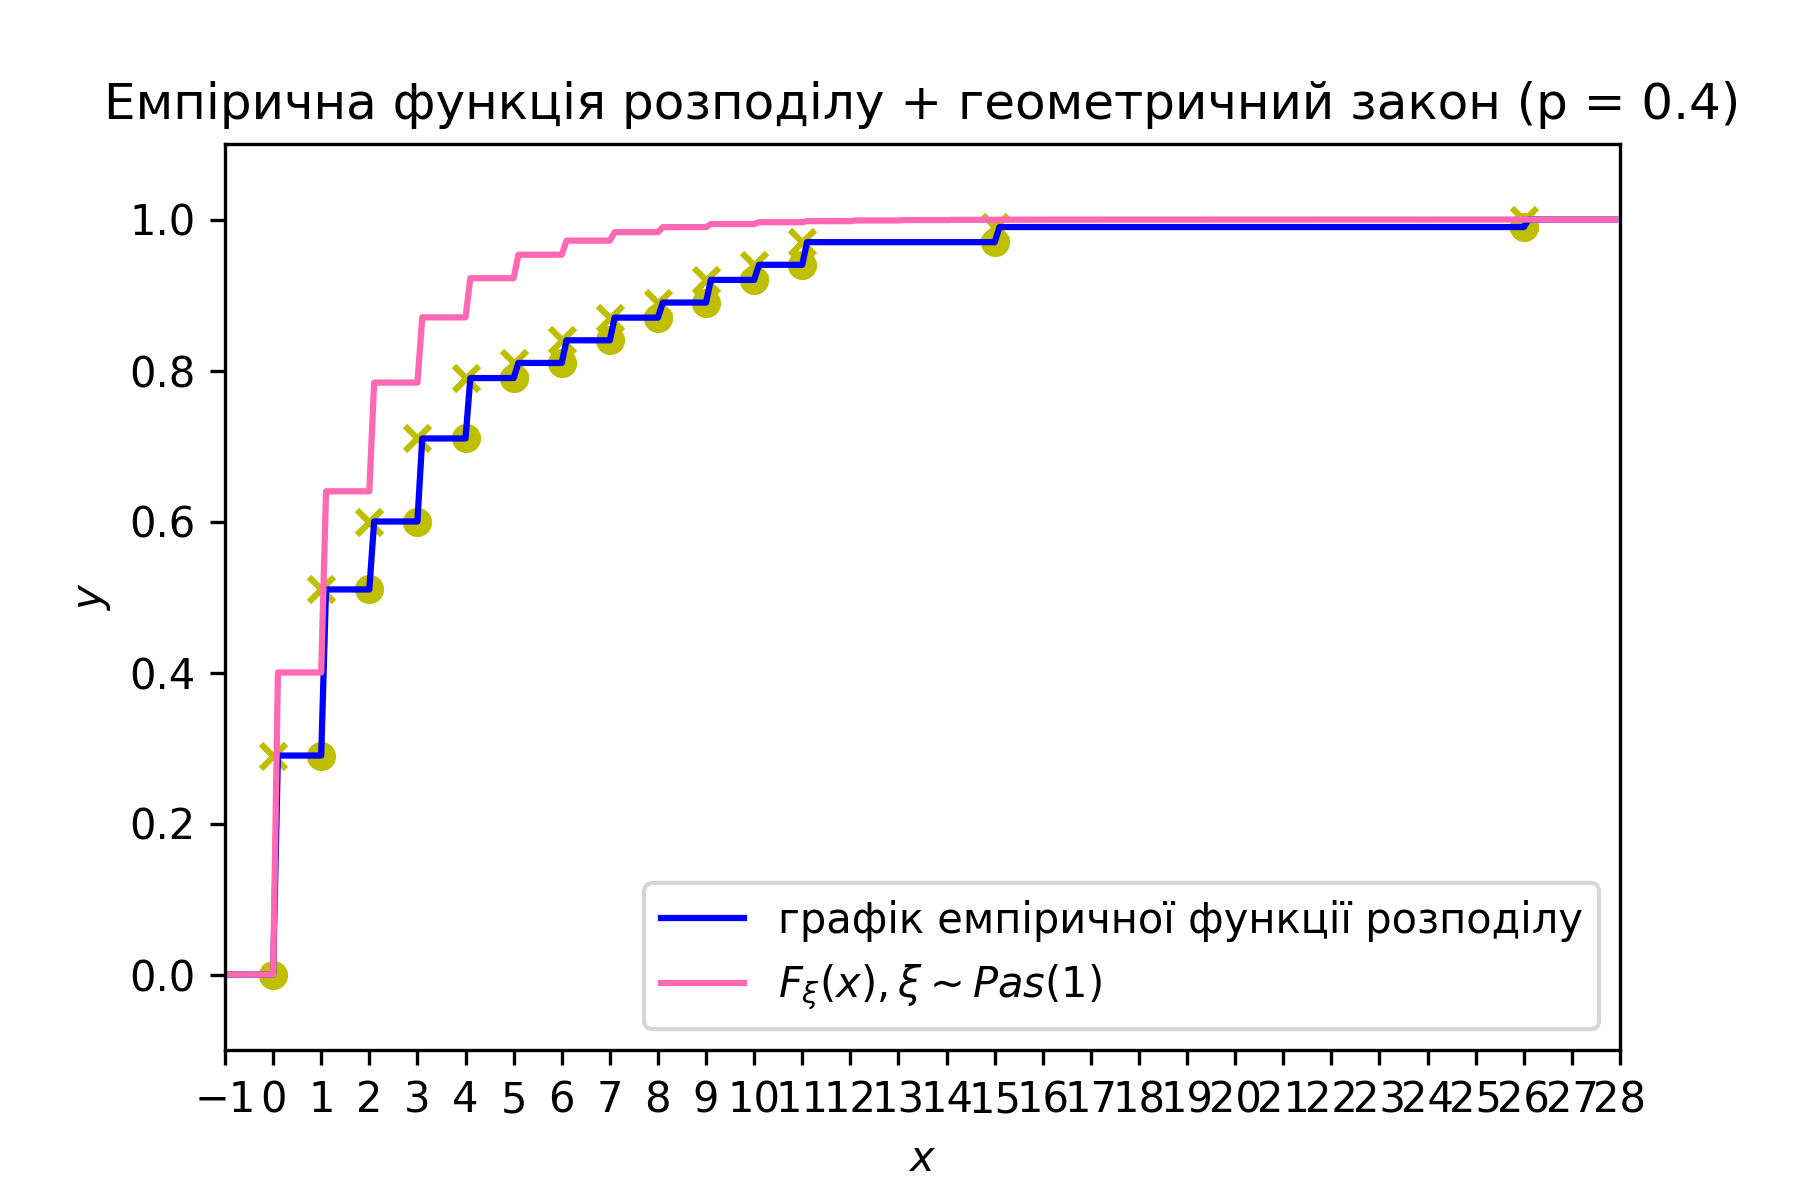
\includegraphics[scale = 0.8]{func+geom4}
\newline
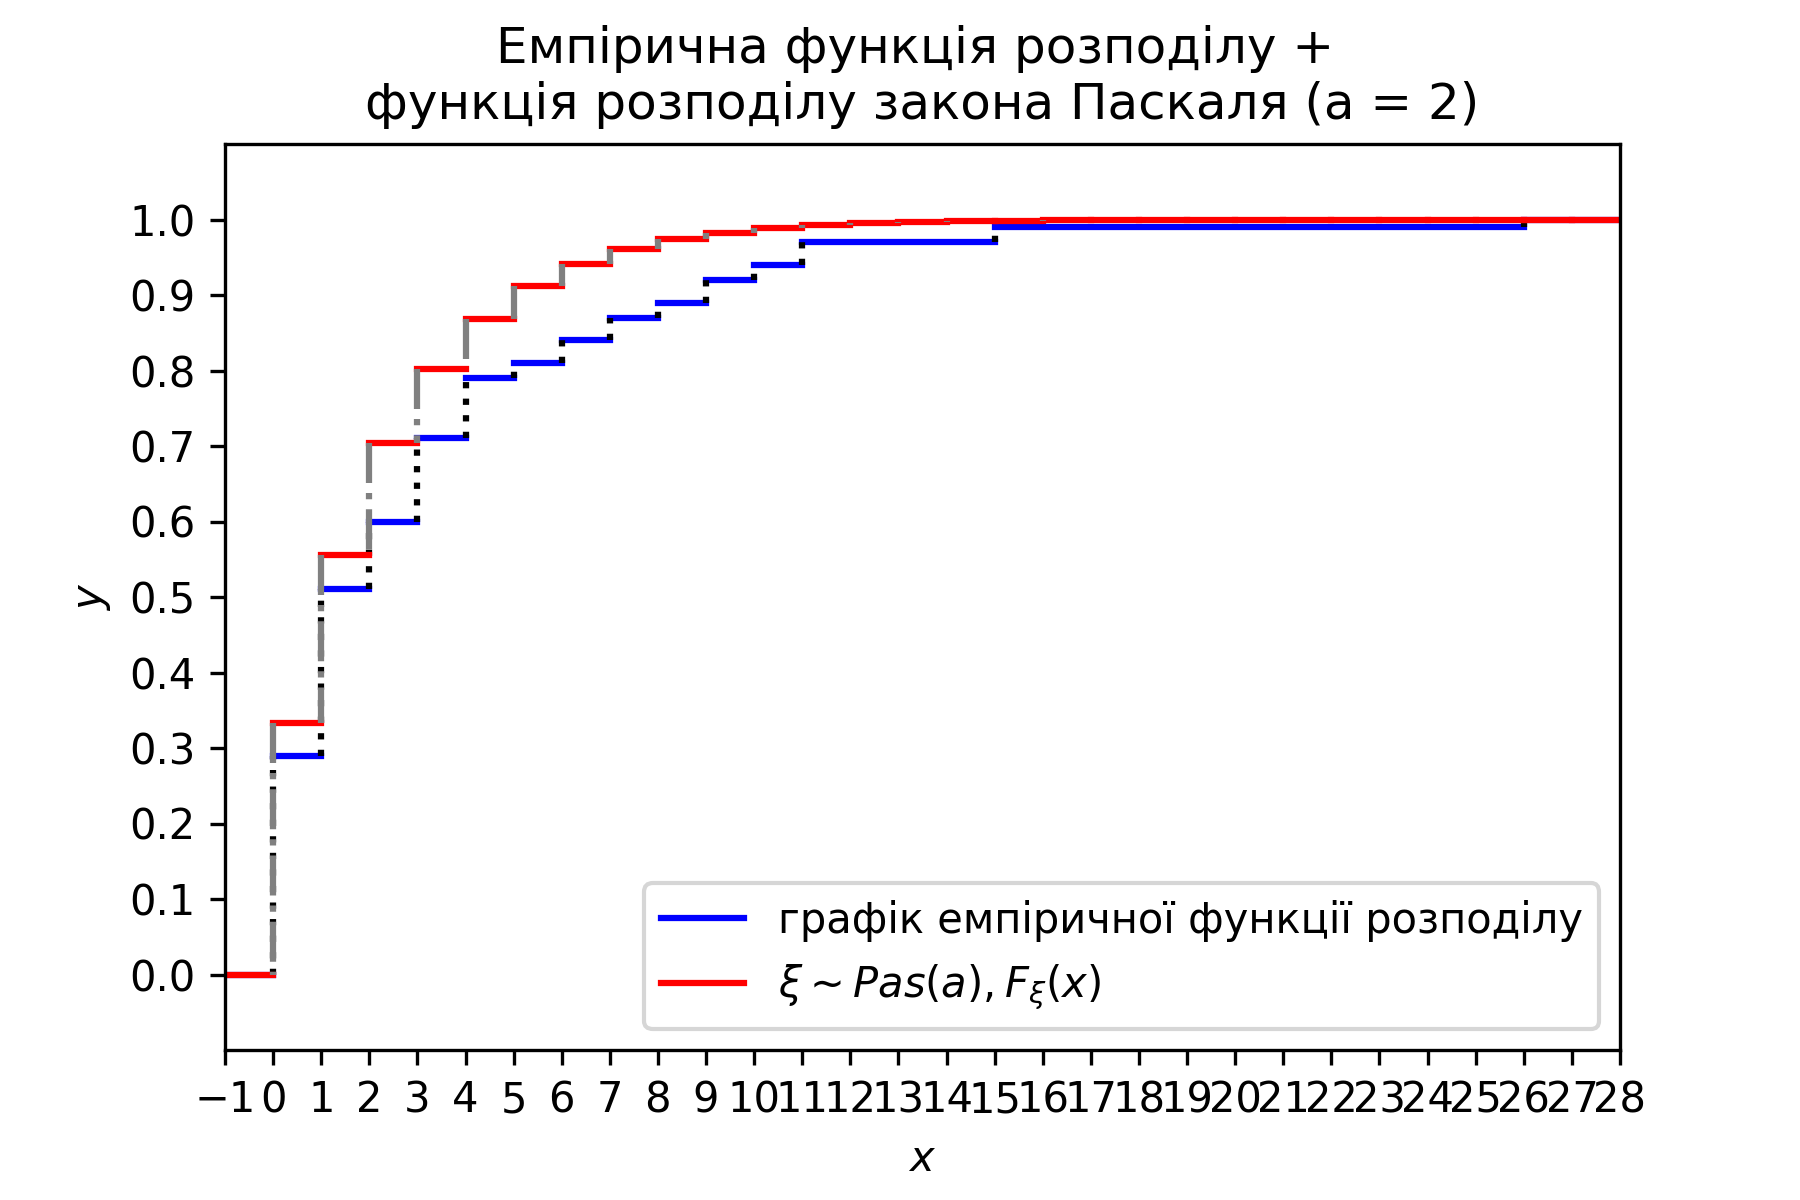
\includegraphics[scale = 0.8]{func+geom3}
\newline
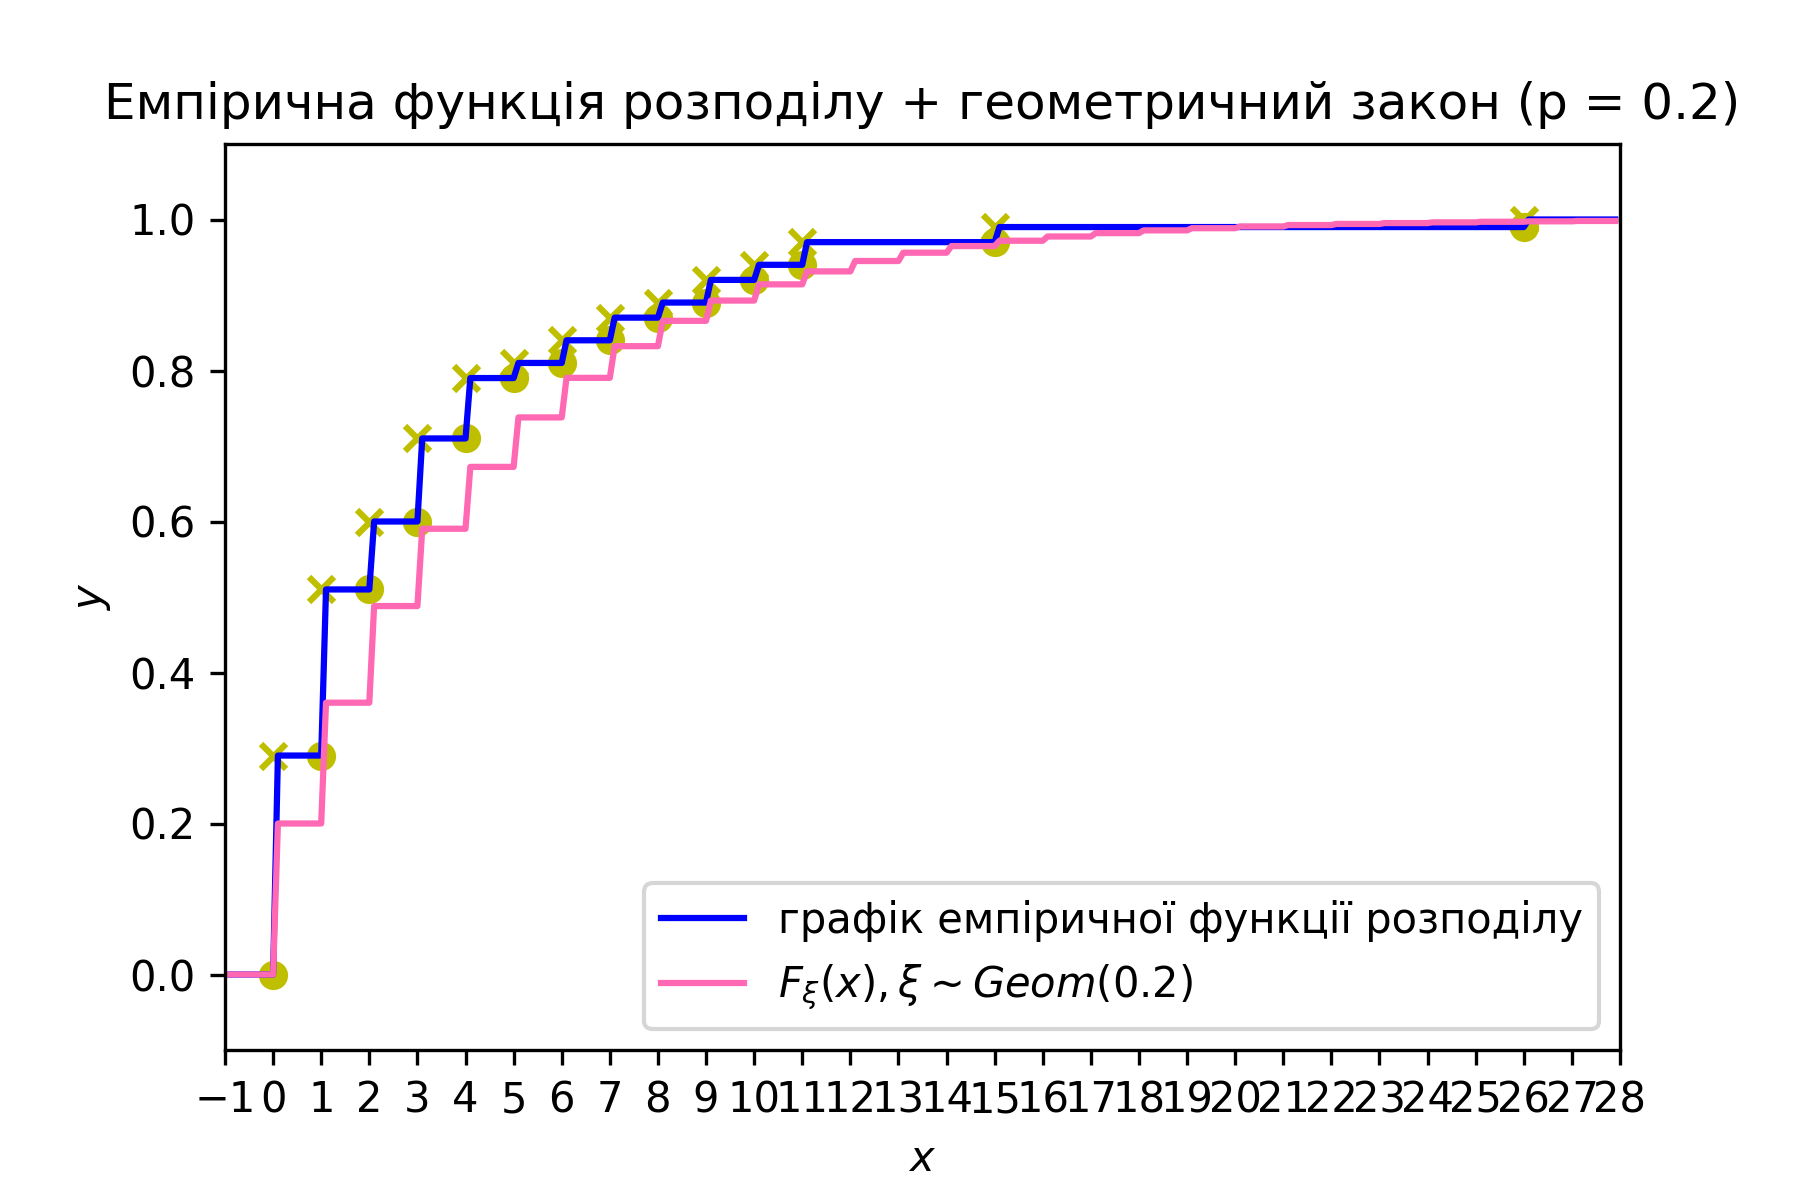
\includegraphics[scale = 0.8]{func+geom2}
\newline
З рисунків вище можна побачити що графік емпіричної функції
розподілу нашої реалізації вибірки схожа при певних значеннях
параметра p на функцію розподілу геометричного закону зі 
значеннями $\in \{ 0, 1, 2, \dots \} $.
\section{Обчислення вибіркових характеристик генеральної 
сукупності (медіана, мода, ассиметрія)}
Для початку знайдемо $({Mo}_\xi^*)_{\text{знач.}}$ - 
значення вибіркової моди (тієї варіанти, якій відповідає 
найбільша частість). Для знаходження цієї варіанти використаємо
вже побудований дискретний варіаційний ряд (див. ст. 1 пункт 2).
Проаналізувавши варіаційний ряд побачимо, що:
$$({Mo}_\xi^*)_{\text{знач.}} = x_1^* = 0$$
Зауважимо, що випадкова величина $\mu$, розподілена за 
геометричним закон при будь-яких значеннях параметра p
має моду ${Mo}_\mu = 0$.
\newline
\newline
Знайдемо значення вибіркової медіани $({Me}_\xi^*)_{\text{знач.}}$ 
для нашої реалізації виборки. З варіаційного ряду (див. ст. 1 
пункт 2), враховуючи те що кількість варіант - парна, 
знайдемо:$$ ({Me}_\xi^*)_{\text{знач.}} = \frac{x_7^* + x_8^*}
{2} = 6.5 $$
\newline
Для знаходження значення вибіркової ассиметрія спочатку потрібно 
знайти значення вибіркової дисперсії, а тому й вибіркового середнього: 
$$\overline{x} = (E^*_{\xi})_{\text{знач.}} = \frac{1}{100} 
\sum_{k = 1}^{14} x_k^* n_k = 3.06$$
За допомогою цього знайдемо значення вибіркової дисперсії:
$$(D^*_{\xi})_{\text{знач.}} = \frac{1}{100} \sum_{k = 1}^{100}
(x_k - 3.06)^2 = 17.136400000000002$$
Отримавши значення вибіркової дисперсії, можна отримати значення
вибіркової ассиметрії для даної реалізації вибірки:
$$({As}_{\xi}^*)_{\text{знач.}} = \frac{\frac{1}{100}
\sum_{k = 1}^{100}(x_k - 3.06)^3}{(17.136400000000002)^
{\frac{3}{2}}} = 2.504088773053977$$
\section{Незміщена оцінка математичного сподівання та дисперсії}
\end{document}
